\section{Les catégories: premier contact}

%%%%%%%%%%%%%%%%%%%%%%%%%%%%%%%%%%%%%%%%%%%%%%%%%%%%%%%%%%%%%%%%%%%%%%%%%%%%%%
\subsection{Définition formelle}
Une catégorie $\C$ est composée de trois choses:
\begin{enumerate}
    \item Une collection d'objets, habituellement notée $\ob(\C)$.
    \item Une collection de flèches (aussi appelées morphismes) entre ces
          objets, habituellement notée $\hom(\C)$.
    \item Une opération binaire, habituellement notée $\circ$, permettant de
          composer n'importe quelle paire de flèches dont les sources et
          destinations sont compatibles pour en obtenir une troisième.
\end{enumerate}

Pour que $\C$ soit une catégorie, ces ``choses'' doivent aussi respecter
certaines propriétés, qui seront expliquées un peu plus bas. Avant de
continuer, il est important de préciser quelques détails et d'introduire
un peu de notation qui rendra notre tâche plus facile pour la suite. D'abord,
pour deux objets $X, Y \in \ob(\C)$, on note la collection des flèches allant
de $X$ vers $Y$ par $\hom(X, Y)$, ou encore $\hom_\C(X, Y)$ lorsque la catégorie
$\C$ n'est pas évidente à partir du contexte. On utilise aussi la notation
$f : X \to Y$ pour dire que $f$ est une flèche allant de $X$ vers $Y$,
c'est-à-dire que $f \in \hom(X, Y)$. On dit alors que $f$ est de source
$X$ et de destination $Y$, noté $\dom(f)$ et $\range(f)$ respectivement.

Ensuite, il est important de bien comprendre qu'on ne parle pas en réalité
d'une seule opération binaire, mais bien d'une opération binaire pour chaque
triplet d'objets $X, Y, Z \in \ob(\C)$. En effet, on souhaite définir notre
opération binaire de manière à ce qu'elle puisse composer n'importe quelles
deux flèches dont les sources et destinations sont compatibles, c'est-à-dire
que pour des flèches $f : Y \to Z$ et $g : X \to Y$, on puisse écrire
$f \circ g$. La définition de $\circ$ doit donc être de la forme
\begin{align*}
    \circ : \hom(Y, Z) \times \hom(X, Y) &\to \hom(X, Z) \\
             f, g &\mapsto f \circ g
\end{align*}

Il est donc nécessaire de parler d'une telle opération $\circ$ pour chaque
paire de $\hom$-classe $\left(\hom(Y, Z), \hom(X, Y)\right)$, ou, de manière
équivalente, pour chaque triplet d'objets $\left(X, Y, Z\right)$. Pour justifier
rigoureusement notre abus de langage, appelons $\circ_{\left(X,Y,Z\right)}$
l'opération binaire associée au triplet d'objets $\left(X,Y,Z\right)$.
Il suffit maintenant de définir la composition comme
\begin{align*}
    \circ : \bigcup \left\{ \dom(\circ_{\left(X,Y,Z\right)})
                            \suchthat X, Y, Z \in \ob(\C) \right\} &\to \hom(\C) \\
           f, g &\mapsto f \circ_{\left(\dom(g), \range(g), \range(f)\right)} g
\end{align*}
, ce qui nous permet de composer n'importe quelles deux flèches dont les sources
et destinations sont compatibles sans s'enfarger dans les fleurs du tapis. Nous
sommes maintenant prêts à passer aux propriétés qui doivent être satisfaites
pour qu'on ait bien une catégorie. D'abord, pour tout objet $X \in \ob(\C)$,
il doit exister une flèche de $X$ vers lui-même, qu'on appelle généralement
identité (sur $X$):
\[
    \id_X : X \to X
\]

Ensuite, la composition $\circ$ définie plus haut doit être associative,
c'est-à-dire que pour toutes flèches $f : C \to D$, $g : B \to C$ et
$h : A \to B$, on doit avoir
\[
    (f \circ g) \circ h = f \circ (g \circ h)
\]

Finalement, on doit avoir que les identités sont des éléments neutres de la
composition, c'est-à-dire que pour toute flèche $f : A \to B$,
\[
    f = \id_B \circ f = f \circ \id_A
\]

Il est intéressant d'observer que ces deux dernières propriétés sont
semblables à demander que $\left(\hom(\C), \circ\right)$ soit un monoïde.
Ce n'est évidemment pas le cas puisqu'on a plusieurs identités et parce
que $\circ$ n'est pas définie sur la totalité de $\hom(\C) \times \hom(\C)$,
mais l'intuition reste utile.


%%%%%%%%%%%%%%%%%%%%%%%%%%%%%%%%%%%%%%%%%%%%%%%%%%%%%%%%%%%%%%%%%%%%%%%%%%%%%%
\subsection{Exemples de catégories}
Avec la définition d'une catégorie qui vient d'être faite, il est un peu
difficile de voir comment les catégories peuvent se matérialiser. Nous
explorerons donc maintenant des catégories simples qui permettent de se
forger une intuition dans le but éventuel d'étudier des catégories plus utiles.
Dans cet optique, on se doit de commencer par la catégorie la plus simple;
la catégorie vide. Comme son nom l'indique, cette catégorie n'a pas d'objets
ni de flèches, et sa loi de composition est une application vide
$\circ : \emptyset \times \emptyset \to \emptyset$. Les propriétés d'une
catégorie sont trivialement satisfaites. Une autre catégorie simple (et
peu utile) est la catégorie triviale, qui ne contient qu'un seul objet
et sa flèche identité:

\centerline{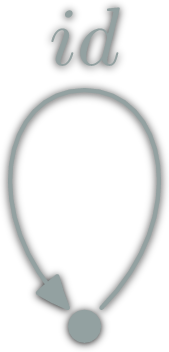
\includegraphics[scale=0.3]{figures/trivial}}

De manière générale, on peut voir une catégorie comme un graphe dirigé avec
certaines propriétés. Par exemple, le graphe suivant est une catégorie:

% TODO
\centerline{\tikz \draw (0,0) rectangle (3, 2);}

Les objets sont les sommets du graphe, les flèches sont les arrêtes et la loi
de composition est une application qui associe à deux arrêtes $u$ et $v$ un
troisième sommet qui part de la source de $u$ jusqu'à la destination de $v$.
Bien entendu, tous les graphes ne sont pas des catégories. Par exemple, le
graphe suivant ne peut pas être une catégorie:

% TODO
\centerline{\tikz \draw (0,0) rectangle (3, 2);}

En effet, il n'y a pas d'arrête qui part du sommet $a$ vers lui-même, ce qui
ne respecte pas le fait que chaque objet doit avoir une flèche identité. Aussi,
bien qu'il respecte les identités, le graphe suivant ne peut pas être une
catégorie:

% TODO
\centerline{\tikz \draw (0,0) rectangle (3, 2);}

En effet, il existe une arrête entre les sommets $a$ et $b$ et une arrête
entre les sommets $b$ et $c$, mais il n'y en a pas entre les sommets $a$ et
$c$. Si on essayait de définir la loi de composition, on se rendrait compte
qu'il n'y a pas de valeur possible pour $u \circ v$. Ainsi, la composition
serait mal définie et le graphe ne peut pas représenter une catégorie. En
général, on peut créer une catégorie à partir de n'importe quel graphe dirigé
en ajoutant simplement les flèches manquantes.

Une des raisons d'étudier les catégories est leur capacité d'unifier des
notions sous un même emblème. Suivant cette ligne de pensée, il est possible
d'inscrire la plupart des structures provenant de l'algèbre abstraite dans
un contexte catégorique. On commence d'abord par la catégorie $\mathrm{Set}$,
dont les objets sont les ensembles, les flèches sont les applications
ensemblistes et la composition est la composition usuelle de fonctions.
On peut ensuite ajouter de la structure à ces ensembles et demander que
les applications ensemblistes respectent cette structure. Ceci nous mène
à considérer, par exemple, la catégorie $\mathrm{Grp}$, où les objets sont
les groupes et les flèches sont des homomorphismes de groupe, avec la
composition usuelle. On peut continuer sur ce chemin et considérer la
catégorie $\mathrm{Ring}$ des anneaux, où les flèches sont des homomorphismes
d'anneaux, puis la catégorie $\mathrm{K-Vect}$ des espaces vectoriels sur un
corps $K$, où les flèches sont les transformations K-linéaires, et ainsi de
suite. Du côté de l'analyse, on peut considérer par exemple la catégorie
$\mathrm{Met}$ des espaces métriques, où les flèches sont les applications
1-Lipschitz. Les exemples sont nombreux; en fait, la plupart des théories
mathématiques peuvent être exprimés dans ce cadre, parfois moyennant une
petite dose d'imagination.


%%%%%%%%%%%%%%%%%%%%%%%%%%%%%%%%%%%%%%%%%%%%%%%%%%%%%%%%%%%%%%%%%%%%%%%%%%%%%%
\subsection{La catégorie Hask}

